% Options for packages loaded elsewhere
\PassOptionsToPackage{unicode}{hyperref}
\PassOptionsToPackage{hyphens}{url}
\documentclass[
]{article}
\usepackage{xcolor}
\usepackage[margin=1in]{geometry}
\usepackage{amsmath,amssymb}
\setcounter{secnumdepth}{-\maxdimen} % remove section numbering
\usepackage{iftex}
\ifPDFTeX
  \usepackage[T1]{fontenc}
  \usepackage[utf8]{inputenc}
  \usepackage{textcomp} % provide euro and other symbols
\else % if luatex or xetex
  \usepackage{unicode-math} % this also loads fontspec
  \defaultfontfeatures{Scale=MatchLowercase}
  \defaultfontfeatures[\rmfamily]{Ligatures=TeX,Scale=1}
\fi
\usepackage{lmodern}
\ifPDFTeX\else
  % xetex/luatex font selection
\fi
% Use upquote if available, for straight quotes in verbatim environments
\IfFileExists{upquote.sty}{\usepackage{upquote}}{}
\IfFileExists{microtype.sty}{% use microtype if available
  \usepackage[]{microtype}
  \UseMicrotypeSet[protrusion]{basicmath} % disable protrusion for tt fonts
}{}
\makeatletter
\@ifundefined{KOMAClassName}{% if non-KOMA class
  \IfFileExists{parskip.sty}{%
    \usepackage{parskip}
  }{% else
    \setlength{\parindent}{0pt}
    \setlength{\parskip}{6pt plus 2pt minus 1pt}}
}{% if KOMA class
  \KOMAoptions{parskip=half}}
\makeatother
\usepackage{longtable,booktabs,array}
\usepackage{calc} % for calculating minipage widths
% Correct order of tables after \paragraph or \subparagraph
\usepackage{etoolbox}
\makeatletter
\patchcmd\longtable{\par}{\if@noskipsec\mbox{}\fi\par}{}{}
\makeatother
% Allow footnotes in longtable head/foot
\IfFileExists{footnotehyper.sty}{\usepackage{footnotehyper}}{\usepackage{footnote}}
\makesavenoteenv{longtable}
\usepackage{graphicx}
\makeatletter
\newsavebox\pandoc@box
\newcommand*\pandocbounded[1]{% scales image to fit in text height/width
  \sbox\pandoc@box{#1}%
  \Gscale@div\@tempa{\textheight}{\dimexpr\ht\pandoc@box+\dp\pandoc@box\relax}%
  \Gscale@div\@tempb{\linewidth}{\wd\pandoc@box}%
  \ifdim\@tempb\p@<\@tempa\p@\let\@tempa\@tempb\fi% select the smaller of both
  \ifdim\@tempa\p@<\p@\scalebox{\@tempa}{\usebox\pandoc@box}%
  \else\usebox{\pandoc@box}%
  \fi%
}
% Set default figure placement to htbp
\def\fps@figure{htbp}
\makeatother
\setlength{\emergencystretch}{3em} % prevent overfull lines
\providecommand{\tightlist}{%
  \setlength{\itemsep}{0pt}\setlength{\parskip}{0pt}}
\usepackage{booktabs}
\usepackage{longtable}
\usepackage{array}
\usepackage{multirow}
\usepackage{wrapfig}
\usepackage{float}
\usepackage{colortbl}
\usepackage{pdflscape}
\usepackage{tabularx}
\usepackage{xltabular}
\usepackage{threeparttable}
\usepackage{threeparttablex}
\usepackage[normalem]{ulem}
\usepackage{makecell}
\usepackage{xcolor}
\usepackage{bookmark}
\IfFileExists{xurl.sty}{\usepackage{xurl}}{} % add URL line breaks if available
\urlstyle{same}
\hypersetup{
  pdftitle={ETO5513 Assignment 1 Ayshani Vallabh 30646081},
  hidelinks,
  pdfcreator={LaTeX via pandoc}}

\title{ETO5513 Assignment 1 Ayshani Vallabh 30646081}
\author{}
\date{\vspace{-2.5em}2026-11-06}

\begin{document}
\maketitle

\subsection{Research Question- How does fruit consumption differ
globally?}\label{research-question--how-does-fruit-consumption-differ-globally}

The purpose of this analysis is to examine the differences in fruit
consumption globally across the time period of the last 50 years.
Specifically, the consumption of different groups of fruit will be
analysed in relation to different geographic groups, across continents
and different income levels.

\subsection{Data}\label{data}

The dataset used in this analysis is from Our World in Data, with
original data from FAOSTAT (Food and Agriculture Organization of the
United Nations)(Food and Agriculture Organization of the United
Nations,n.d). The raw data contained 561 rows, with 14 variables. To
reduce the dataset to the size specified for this analysis (at least 3
numerical variables and no more than 5 overall), similar fruits were
grouped and the remaining columns were dropped.

\subsubsection{Variables}\label{variables}

For the purpose of this analysis, two new groups of fruits were created
(Citrus and Apples, Bananas and Oranges) by combining existing
variables, with the remaining variables (excluding `Other Fruits') being
dropped (Geographic code, Dates, Plantains, Pineapples and Grapes). The
rationale behind using these groups was that it included fruits that
seemed to the most common (Apples, Bananas, Oranges), a wider group that
combined a range of similar existing variables (Citrus, which combined
three original variables) and a category that was already present in the
raw data that encompassed various other fruits that have not been listed
separately. The remaining variables represented geographic area (with
the raw data being pre sorted into continent and income group from Our
World in Data and FAOSTAT) and the year.

\texttt{The\ raw\ data\ contained\ 561\ observations\ with\ 14\ variables,\ and\ the\ final\ dataset\ that\ will\ be\ used\ for\ analysis\ contains\ 510\ observations,\ across\ 5\ variables,\ as\ the\ \textquotesingle{}World\textquotesingle{}\ group\ was\ removed.}

\pandocbounded{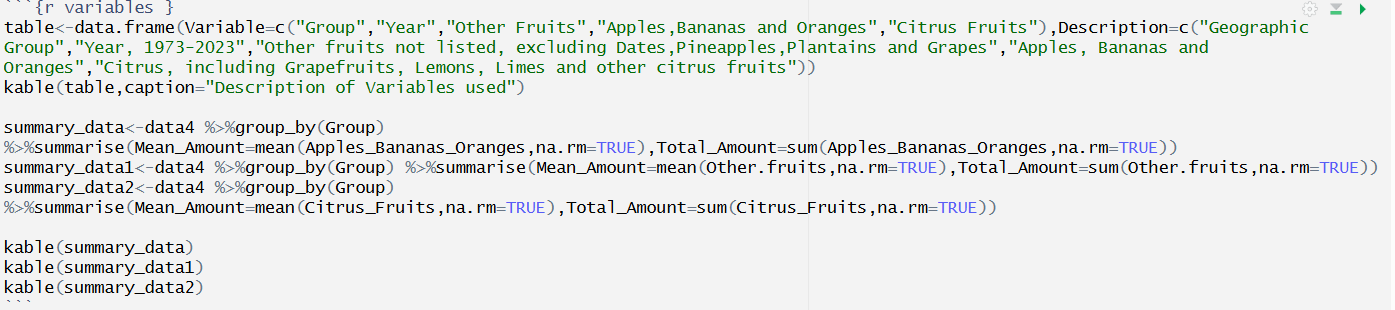
\includegraphics[keepaspectratio]{Screenshot 2026-11-08 155519.png}}

\begin{verbatim}
## 'data.frame':    510 obs. of  5 variables:
##  $ Group                 : chr  "Africa" "Africa" "Africa" "Africa" ...
##  $ Year                  : int  1973 1974 1975 1976 1977 1978 1979 1980 1981 1982 ...
##  $ Other.fruits          : num  11.2 11.5 11.5 11.6 11.4 ...
##  $ Citrus_Fruits         : num  5.97 5.86 5.54 5.4 5.3 ...
##  $ Apples_Bananas_Oranges: num  17.8 18.3 17.5 17.2 16.4 ...
\end{verbatim}

\begin{verbatim}
## Warning: package 'kableExtra' was built under R version 4.5.3
\end{verbatim}

\begin{verbatim}
## 
## Attaching package: 'kableExtra'
\end{verbatim}

\begin{verbatim}
## The following object is masked from 'package:dplyr':
## 
##     group_rows
\end{verbatim}

\begin{longtable}[]{@{}
  >{\raggedright\arraybackslash}p{(\linewidth - 2\tabcolsep) * \real{0.2160}}
  >{\raggedright\arraybackslash}p{(\linewidth - 2\tabcolsep) * \real{0.7840}}@{}}
\caption{Description of Variables used}\tabularnewline
\toprule\noalign{}
\begin{minipage}[b]{\linewidth}\raggedright
Variable
\end{minipage} & \begin{minipage}[b]{\linewidth}\raggedright
Description
\end{minipage} \\
\midrule\noalign{}
\endfirsthead
\toprule\noalign{}
\begin{minipage}[b]{\linewidth}\raggedright
Variable
\end{minipage} & \begin{minipage}[b]{\linewidth}\raggedright
Description
\end{minipage} \\
\midrule\noalign{}
\endhead
\bottomrule\noalign{}
\endlastfoot
Group & Geographic Group \\
Year & Year, 1973-2023 \\
Other Fruits & Other fruits not listed, excluding
Dates,Pineapples,Plantains and Grapes (kg per capita per year) \\
Apples,Bananas and Oranges & Apples, Bananas and Oranges (kg per capita
per year) \\
Citrus Fruits & Citrus, including Grapefruits, Lemons, Limes and other
citrus fruits (kg per capita per year \\
\end{longtable}

\begin{longtable}[]{@{}lrr@{}}
\caption{Mean and Sum of Apples, Bananas and Oranges}\tabularnewline
\toprule\noalign{}
Group & Mean\_Amount & Total\_Amount \\
\midrule\noalign{}
\endfirsthead
\toprule\noalign{}
Group & Mean\_Amount & Total\_Amount \\
\midrule\noalign{}
\endhead
\bottomrule\noalign{}
\endlastfoot
Africa & 20.23927 & 1032.203 \\
Asia & 20.46185 & 1043.554 \\
Europe & 43.37030 & 2211.885 \\
High-income countries & 51.43296 & 2623.081 \\
Low-income countries & 24.16746 & 1232.540 \\
Lower-middle-income countries & 16.36378 & 834.553 \\
North America & 63.60476 & 3243.843 \\
Oceania & 54.42449 & 2775.649 \\
South America & 54.06084 & 2757.103 \\
Upper-middle-income countries & 29.36473 & 1497.601 \\
\end{longtable}

\begin{longtable}[]{@{}lrr@{}}
\caption{Mean and Sum of Other Fruit}\tabularnewline
\toprule\noalign{}
Group & Mean\_Amount & Total\_Amount \\
\midrule\noalign{}
\endfirsthead
\toprule\noalign{}
Group & Mean\_Amount & Total\_Amount \\
\midrule\noalign{}
\endhead
\bottomrule\noalign{}
\endlastfoot
Africa & 12.24470 & 624.4797 \\
Asia & 19.33451 & 986.0599 \\
Europe & 22.81782 & 1163.7087 \\
High-income countries & 21.69611 & 1106.5016 \\
Low-income countries & 12.73997 & 649.7386 \\
Lower-middle-income countries & 17.58224 & 896.6940 \\
North America & 23.31990 & 1189.3149 \\
Oceania & 24.93814 & 1271.8454 \\
South America & 18.68897 & 953.1373 \\
Upper-middle-income countries & 20.54891 & 1047.9943 \\
\end{longtable}

\begin{longtable}[]{@{}lrr@{}}
\caption{Mean and Sum of Citrus Fruits}\tabularnewline
\toprule\noalign{}
Group & Mean\_Amount & Total\_Amount \\
\midrule\noalign{}
\endfirsthead
\toprule\noalign{}
Group & Mean\_Amount & Total\_Amount \\
\midrule\noalign{}
\endhead
\bottomrule\noalign{}
\endlastfoot
Africa & 5.577308 & 284.44272 \\
Asia & 2.154290 & 109.86879 \\
Europe & 3.741798 & 190.83172 \\
High-income countries & 6.245376 & 318.51416 \\
Low-income countries & 1.095600 & 55.87561 \\
Lower-middle-income countries & 2.907187 & 148.26652 \\
North America & 10.572596 & 539.20237 \\
Oceania & 2.887230 & 147.24874 \\
South America & 5.640970 & 287.68947 \\
Upper-middle-income countries & 3.348691 & 170.78325 \\
\end{longtable}

\begin{verbatim}
## `summarise()` has grouped output by 'Decades'. You can override using the
## `.groups` argument.
\end{verbatim}

\begin{longtable}[t]{lrrrrrrrrrr}
\caption{\label{tab:variables}Comparison of Fruit (Apples, Bananas and Oranges) Consumption over Time}\\
\toprule
Decades & Africa & Asia & Europe & High-income countries & Low-income countries & Lower-middle-income countries & North America & Oceania & South America & Upper-middle-income countries\\
\midrule
{}[1970,1980) & 17.55 & 9.82 & 35.80 & 46.59 & 34.31 & 10.05 & 56.44 & 47.41 & 57.66 & 17.18\\
{}[1980,1990) & 18.88 & 12.12 & 37.33 & 51.31 & 35.51 & 11.61 & 65.21 & 51.18 & 53.43 & 19.40\\
{}[1990,2000) & 18.65 & 17.55 & 40.26 & 50.03 & 23.57 & 14.37 & 64.03 & 50.84 & 55.92 & 25.43\\
{}[2000,2010) & 22.30 & 23.39 & 47.90 & 52.70 & 19.38 & 17.63 & 62.86 & 56.64 & 50.82 & 32.53\\
{}[2010,2020) & 21.77 & 30.60 & 50.13 & 51.89 & 15.57 & 22.56 & 61.08 & 62.46 & 54.73 & 41.80\\
\addlinespace
{}[2020,2030) & 23.36 & 34.56 & 51.26 & 59.43 & 13.01 & 25.61 & 79.23 & 58.16 & 51.11 & 46.45\\
\bottomrule
\multicolumn{11}{l}{\rule{0pt}{1em}\textit{Note: }}\\
\multicolumn{11}{l}{\rule{0pt}{1em}The dataset only includes data up to and including 2023.}\\
\end{longtable}

\subsubsection{Analysis of Data}\label{analysis-of-data}

The summary statistics above highlight that the fruit group of
Apples,Oranges and Bananas had the highest mean and sum, with Citrus
fruits having the lowest, significantly less than the other groups
analysed.\textbf{Generally, North America had the highest amounts of
fruit consumption (First globally among Apples,Bananas Oranges and
Citrus fruit,and second overall in Other Fruits), whilst Africa and Asia
tended to have the lowest (with the exception of Citrus Fruits in
Africa).}

The consumption of Apples, Bananas and Oranges have steadily increased
over the last 50 years across Africa, Asia and Europe. North America and
Oceania displayed more fluctuations from decade to decade, however still
had an upward trend. On the other hand, the level of consumption
followed a downwards trend in South America, with most recent amounts
being less than the averages from 1973-2000.This was also true for low
income countries, with remaining income groups showing an upwards trend.

\pandocbounded{\includegraphics[keepaspectratio]{eto5513_files/figure-latex/pressure-1.pdf}}
\pandocbounded{\includegraphics[keepaspectratio]{eto5513_files/figure-latex/pressure-2.pdf}}

The first plot above highlights a relatively strong positive
relationship between Apples,Bananas, Oranges and Citrus Fruits, with
North America having the highest amount of both fruit groups. \emph{Most
geographic groups had a proportionate amount of both fruit groups, with
the exception of Africa (who had higher levels of citrus fruit) and
Oceania (who had higher levels of Apples, Bananas and Oranges)}

The next plot highlights a similar positive trend between Other fruits
and citrus fruits, however data points are more clustered together along
the slope line and more geographic groups displayed a linear trend as
opposed to a cluster shape. As with the previous plot, North America had
the highest levels of citrus fruit; however Oceania had the highest
consumption of other fruit globally. Upper middle income countries had
the highest consumption of other fruits, whilst high income countries
were similar to lower-middle income countries.

Given that other fruit includes berries, stone fruits and tropical
fruits (Food and Agriculture Organization of the United Nations, n.d),
local climates are expected to have a major influence in determining
which more `niche' fruits are grown and therefore consumed.

\subsubsection{Conclusion}\label{conclusion}

Analysis of the data highlights that Apples, Bananas and Oranges are the
most common group, followed by other fruit and citrus fruit. Analysis of
Apples, Bananas and Oranges over time indicated that interestingly,
consumption has not increased across every continent or income
group.This was particularly prevalent in low income countries and in
South America.

North America had a consistently high level of all three fruit groups,
more than most continents. On the other hand, there was no single
continent that consistently low levels of fruits. For example, although
Africa had the lowest amounts of Apples, Bananas, Oranges and Other
fruits, it had the third highest level of citrus fruit.

The relationship between Apples, Bananas, Oranges and Citrus fruits
demonstrated a moderate, positive trend. This suggests that most groups
had a somewhat proportionate level of consumption of the two groups. The
exception to this trend was Africa and Oceania who had much higher
consumption levels of only citrus or apples,bananas and oranges,
respectively. When comparing citrus and other fruits, the relationship
was similar, however the slope was generally more steep and resulted in
almost three branches, with North America and South America showing a
much stronger relationship than Oceania for example, which followed a
slight downwards trend instead.

As expected, high income countries had generally the highest amounts of
all fruits. This is likely to be attributed to the increased ability to
import and perhaps grow a wider range of fruits, however more research
is needed to confirm this assumption. Conversely, lower income countries
had the lowest amounts of citrus and other fruits, however had a higher
amount of Apples, Bananas and Oranges than lower-middle income
countries. To provide more insight, future research could examine
agricultural data in relation to geographic location to determine the
drivers behind these levels of consumption.

\subsubsection{References}\label{references}

Food and Agriculture Organization of the United Nations (2025) --
processed by Our World in Data. ``Yearly per capita supply of dates''
{[}dataset{]}. Food and Agriculture Organization of the United Nations,
``Food Balances: Food Balances (-2013, old methodology and
population)''; Food and Agriculture Organization of the United Nations,
``Food Balances: Food Balances (2010--)'' {[}original data{]}

Food and Agriculture Organization of the United Nations(n.d) \emph{Food
Balances (-2013,old methodology and
population)}\url{https://www.fao.org/faostat/en/\#data/FBSH} Food and
Agriculture Organization of the United Nations(n.d) \emph{Food Balances
(-2010)}\url{https://www.fao.org/faostat/en/\#data/FBS}

\end{document}
